\documentclass{beamer}
\usepackage[utf8]{inputenc}
\usetheme{Madrid}
\usecolortheme{default}
\usepackage{amsmath,amssymb,amsfonts,amsthm}
\usepackage{txfonts}
\usepackage{tkz-euclide}
\usepackage{listings}
\usepackage{adjustbox}
\usepackage{array}
\usepackage{tabularx}
\usepackage{gvv}
\usepackage{lmodern}
\usepackage{circuitikz}
\usepackage{tikz}
\usepackage{graphicx}

\setbeamertemplate{page number in head/foot}[totalframenumber]

\usepackage{tcolorbox}
\tcbuselibrary{minted,breakable,xparse,skins}



\definecolor{bg}{gray}{0.95}
\DeclareTCBListing{mintedbox}{O{}m!O{}}{%
  breakable=true,
  listing engine=minted,
  listing only,
  minted language=#2,
  minted style=default,
  minted options={%
    linenos,
    gobble=0,
    breaklines=true,
    breakafter=,,
    fontsize=\small,
    numbersep=8pt,
    #1},
  boxsep=0pt,
  left skip=0pt,
  right skip=0pt,
  left=25pt,
  right=0pt,
  top=3pt,
  bottom=3pt,
  arc=5pt,
  leftrule=0pt,
  rightrule=0pt,
  bottomrule=2pt,
  toprule=2pt,
  colback=bg,
  colframe=orange!70,
  enhanced,
  overlay={%
    \begin{tcbclipinterior}
    \fill[orange!20!white] (frame.south west) rectangle ([xshift=20pt]frame.north west);
    \end{tcbclipinterior}},
  #3,
}
\lstset{
    language=C,
    basicstyle=\ttfamily\small,
    keywordstyle=\color{blue},
    stringstyle=\color{orange},
    commentstyle=\color{green!60!black},
    numbers=left,
    numberstyle=\tiny\color{gray},
    breaklines=true,
    showstringspaces=false,
}
%------------------------------------------------------------
%This block of code defines the information to appear in the
%Title page
\title %optional
{4.4.22}

%\subtitle{A short story}

\author % (optional)
{RATHLAVATH JEEVAN -AI25BTECH11026}



\begin{document}


\frame{\titlepage}
\begin{frame}{Question}
Find the equation of a plane which passes through the point $(3,2,0)$ and contains the line
\begin{align}
\frac{x-3}{1} \;=\; \frac{y-6}{5} \;=\; \frac{z-4}{4}.
 \end{align}
\end{frame}
\begin{frame}{Theoretical Solution}
\textbf{Solution:}\\
 \textbf{Given:}  
\textbf{Finding the plane using column vectors.}


Let the normal be \(\vec{n}=(a,b,c)^T\). We use the form
\begin{align}
\vec{n}^T\vec{x}=1.
\end{align}

The plane passes through the point \(P=(3,2,0)\) and contains the line
\begin{align}
\frac{x-3}{1}=\frac{y-6}{5}=\frac{z-4}{4},
\end{align}
so take a point on the line \(A=(3,6,4)\) and the direction vector
\(\vec{v}=(1,5,4)\).

The conditions are
\begin{align}
\vec{n}^T \vec{P} = 1
\end{align}
\end{frame}

\begin{frame}{Theoretical Solution}
\begin{align}
\vec{n}^T \vec{A} = 1
\end{align}
\begin{align}
\vec{n}^T \vec{v} = 0.
\end{align}

Put these three column vectors together into a matrix (columns are the given points/vectors):

\end{frame}
\begin{frame}{Theoretical Solution}
\begin{align}
\vec{M}=\begin{myvec}{
3 & 3 & 1\\[4pt]
2 & 6 & 5\\[4pt]
0 & 4 & 4}
\end{myvec}
\qquad\text{(columns are }\vec{P},\;\vec{A},\;\vec{v}\text{).}
\end{align}

Then the three scalar conditions above read compactly as
\end{frame}
\begin{frame}{Theoretical Solution}
\begin{align}
\vec{M}=\begin{myvec}{
3 & 3 & 1\\[4pt]
2 & 6 & 5\\[4pt]
0 & 4 & 4}
\end{myvec}
\qquad\text{(columns are }P,\;A,\;\vec{v}\text{).}
\end{align}

Then the three scalar conditions above read compactly as
\begin{align}
\vec{n}^T\vec{M} = \begin{myvec}{1 & 1 & 0}\end{myvec}.
\end{align}
Transposing both sides gives a standard linear system for \(\vec{n}\):
\begin{align}
\vec{M}^T \vec{n} = \begin{myvec}{1\\[4pt]1\\[4pt]0}\end{myvec}.
\end{align}
\end{frame}
\begin{frame}{Theoretical Solution}
Write this out:
\begin{align}
\begin{myvec}{
3 & 2 & 0\\[4pt]
3 & 6 & 4\\[4pt]
1 & 5 & 4
}\end{myvec}
\begin{myvec}{a\\[4pt]b\\[4pt]c}\end{myvec}
=
\begin{myvec}{1\\[4pt]1\\[4pt]0}\end{myvec}.
\end{align}
\begin{align}
\vec{n}
=
\begin{myvec}{1\\-1\\1}\end{myvec}.
\end{align}

Thus a convenient normal vector is \(\vec{n}=(1,-1,1)^T\), and the plane equation in the requested form is
\begin{align}
\begin{myvec}{1\\-1\\1}^T\end{myvec}\vec{x}=1
\end{align}
\end{frame}
\begin{figure}[h!]
    \centering
    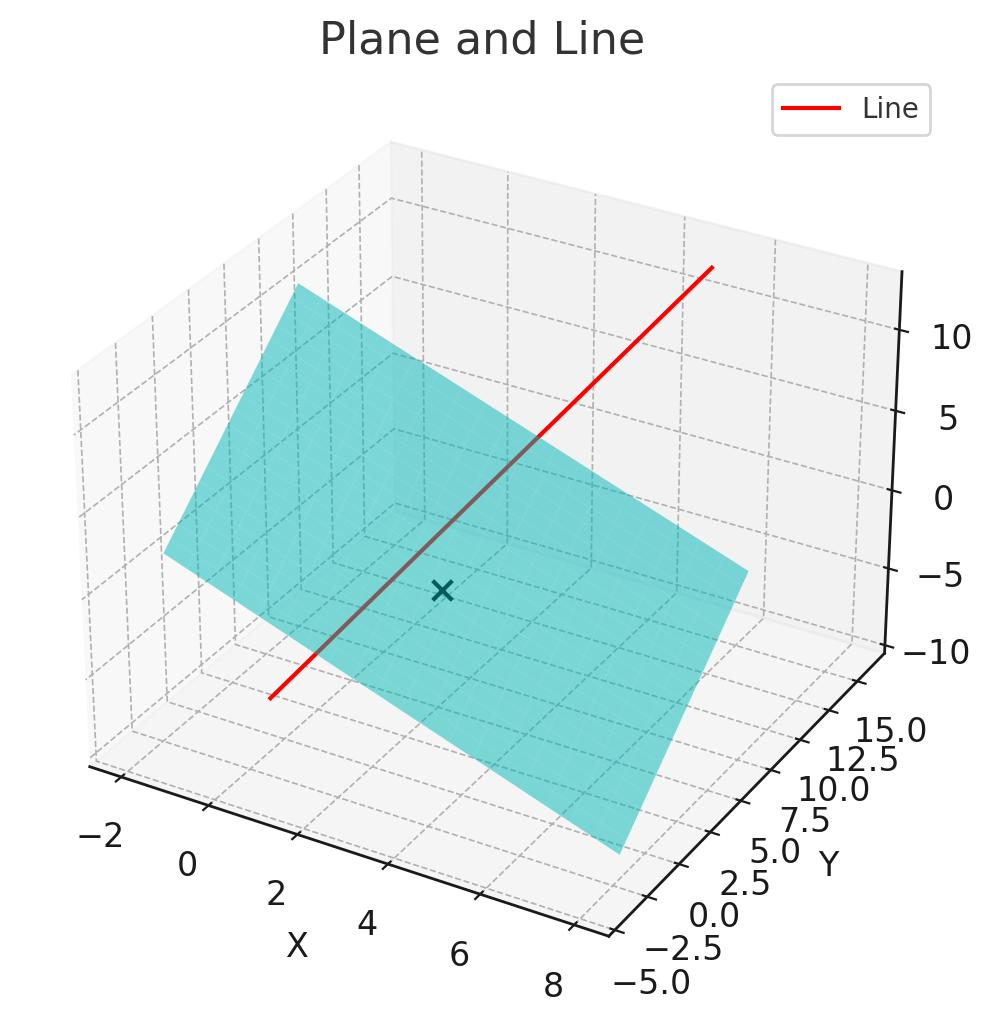
\includegraphics[width=0.5\linewidth]{figs/mat7.jpeg}
    \caption{Caption}
    \label{fig:placeholder}
\end{figure}
\end{document}
